%        File: paper.tex
%     Created: Fri Jun 23 06:00 PM 2017 J
% Last Change: Fri Jun 23 06:00 PM 2017 J
%
\input{../EMSOFT2016/dummy/dummy.tex}
\documentclass[submit]{ipsj_v2/UTF8/ipsj}

\usepackage{latexsym}
\usepackage[dvipdfmx]{graphicx}
\usepackage{amssymb}
\usepackage{enumerate,cite,url}
\usepackage{listings,jlisting}
\lstset{%
    language={c},%
    basicstyle={\small},%
    identifierstyle={\small},%
    commentstyle={\scriptsize\itshape},%
    keywordstyle={\small},%\bfseries},%
    ndkeywordstyle={\small},%
    stringstyle={\small\it},
    frame={tb},
    breaklines=true,
    columns=[l]{fullflexible},%
    numbers=left,%
    xrightmargin=0zw,%
    xleftmargin=3zw,%
    numberstyle={\scriptsize},%
    stepnumber=1,
    numbersep=1zw,%
    lineskip=-1.5ex%
}

\def\Underline{\setbox0\hbox\bgroup\let\\\endUnderline}
\def\endUnderline{\vphantom{y}\egroup\smash{\underline{\box0}}\\}
\def\|{\verb|}

\setcounter{巻数}{53}%vol53=2012
\setcounter{号数}{10}
\setcounter{page}{1}

\begin{document}

\title{組込みシステムに適した動的メモリアロケータのコンポーネント化}

\etitle{Componentized Dynamic Memory Allocator for Embedded Systems}

\affiliate{OU}{大阪大学基礎工学研究科\\
School of Engineering Science, Osaka University}

\affiliate{OKUMA}{オークマ株式会社\\
OKUMA Corporation}

\author{山本 拓朗}{Takuro Yamamoto}{OU}%[joho.taro@ipsj.or.jp]
\author{大山 博司}{Hiroshi Oyama}{OKUMA}%
\author{安積 卓也}{Takuya Azumi}{OU}%[gakkai.jiro@ipsj.or.jp]

\maketitle

\section{はじめに}

\section{基礎技術}
\label{sec:Background}

\subsection{TLSF}

\subsection{TECS}
%TECSは,組込みシステム向けのコンポーネントシステムである.
TECSによるコンポーネントベース開発は,ソフトウェアの再利用性を上げるため,生産性を向上できる.
%システム全体の構造を可視化するため,システムの難しさを減らすことができる.
%ソフトウェアの共通部分はコンポーネントとして扱われるため,開発の重複を減らし,生産性を向上させる.

% TECSでのコンポーネントの生成と結合は静的に行われるため,最適化され,実行時間や消費メモリのオーバヘッドは少ない.
% 他の特徴として,C言語での実装,ソースレベルでの移植性,コンポーネントの粒度が小さいことなどがある.

\subsubsection{コンポーネントモデル}
図\ref{fig:component}にコンポーネント図の例を示す.
TECSでは,インスタンス化されたコンポーネントはセル({\it cell})と呼ばれ,受け口({\it entry}),呼び口({\it call}),属性,変数を持つ.
受け口は自身の機能を提供するインタフェースで,呼び口は他のセルの機能を利用するためのインタフェースである.
セルは複数の受け口や呼び口を持つことができる.
セルの提供する関数は,C言語で実装される.

受け口と呼び口の型は,セルの機能を使うためのインタフェースであるシグニチャによって定義される.
セルの呼び口は,同じシグニチャを持つ他のセルの受け口と結合できる.
セルの型は,セルタイプと呼ばれ,受け口,呼び口,属性,変数の組を定義している.

\begin{figure}[t]
    \centering
    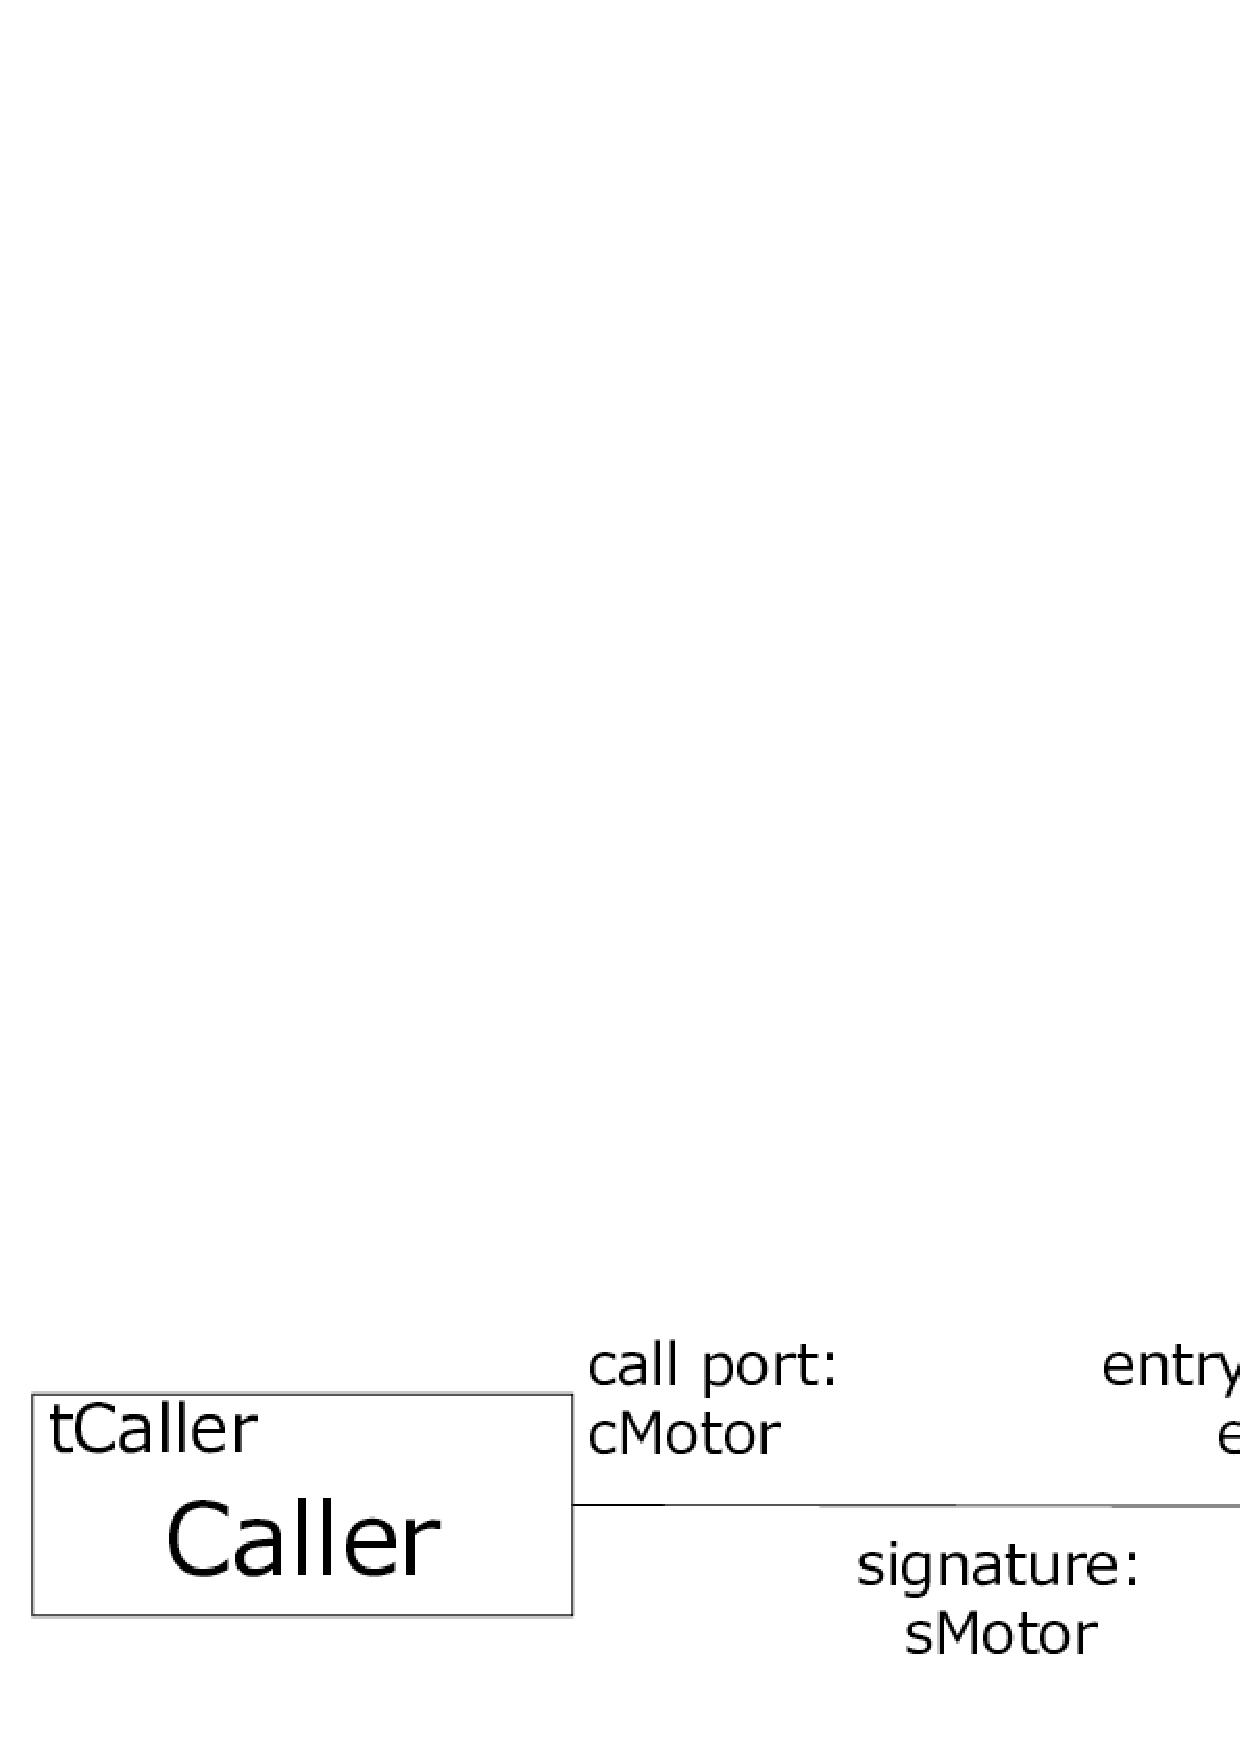
\includegraphics[width=8cm,clip]{../EMSOFT2016/figure/component_diagram.pdf}
    \caption{TECSコンポーネント図の例}
    \label{fig:component}
\end{figure}

\subsubsection{コンポーネント記述}
TECSのコンポーネント記述は,シグニチャ記述,セルタイプ記述,組上げ記述に分類され,cdlファイルに記述する.
図\ref{fig:component}のコンポーネント記述について次に述べる.

% \begin{description}
%     \item[{\bf シグニチャ記述}]\mbox{}\\
        シグニチャ記述は,セルのインタフェースを定義する.
        図\ref{signature}に示す通り,{\it signature}キーワードに続けて,シグニチャ名(sMotor)を記述する.
        %図\ref{signature}のようにシグニチャsMotorを定義できる.
        TECSでは,インタフェースの定義を明確にするために,入力と出力にはそれぞれ,[in]と[out]という指定子が付けられる.
        
\begin{figure}[t]
\centering
\begin{lstlisting}
signature sMotor{
    int32_t getCounts( void );
    ER resetCounts( void );
    ER setPower( [in]int power );
    ER stop( [in] bool_t brake );
    ER rotate( [in] int degrees, [in] uint32_t speed_abs,
              [in] bool_t blocking );
    void initializePort( [in]int32_t type );
};
\end{lstlisting}
\caption{シグニチャ記述}
\label{signature}
\end{figure}

    % \item[{\bf セルタイプ記述}]\mbox{}\\
        セルタイプ記述は,受け口,呼び口,属性,変数を用いてセルタイプを定義する.
        {\it celltype}キーワードに続けて,セルタイプ名(tCaller)を記述する.
        図\ref{celltype}に示す通り,受け口は,{\it entry}キーワードに続けて,シグニチャ名,受け口名を記述する.
        同様にして,呼び口も定義できる.
        属性と変数は,それぞれ{\it attr},{\it var}キーワードを用いて列挙する.

\begin{figure}[t]
\centering
\begin{lstlisting}
celltype tCaller{
    call sMotor cMotor;
};
celltype tMotor{
    entry sMotor eMotor;
    attr{ int32_t attr = 100; };
    var{ int32_t var; };
};
\end{lstlisting}
\caption{セルタイプ記述}  
\label{celltype}
\end{figure}

    % \item[{\bf 組上げ記述}]\mbox{}\\
        組上げ記述は,セルをインスタンス化し,セルを結合する.
        {\it cell}キーワードに続けて,セルタイプ名,セル名を記述する.
        呼び口名,``=",結合先の受け口名の順に記述し,セルを結合する.
        図\ref{build}では,セルCallerの呼び口cMotorと,セルMotorの受け口eMotorが接続されている.
        
\begin{figure}[t]
\centering
\begin{lstlisting}
cell tMotor Motor{
};
cell tCaller Caller{
    cMotor = Motor.eMotor;
};
\end{lstlisting}
\caption{組上げ記述}
\label{build}
\end{figure}

% \end{description}

\section{設計と実装}
\label{sec:Design and Implementation}


\section{評価実験}
\label{sec:Evaluation}

\section{関連研究}
\label{sec:Related Work}

\section{おわりに}
\label{sec:Conclusion}

%%%%%%%%%%%% Reference %%%%%%%%%%%%%%%%%%%%%%%%%%%%%%%%%%%%%%%%%%%%%%
\bibliographystyle{ipsj_v2/UTF8/ipsjunsrt-e}
\bibliography{ref}

% \begin{biography}
% \profile{m,E}{情報 太郎}{1970年生.1992年情報処理大学理学部情報科学科卒業.
% 1994年同大学大学院修士課程修了.同年情報処理学会入社.オンライン出版の研究
% に従事.電子情報通信学会,IEEE,ACM 各会員.}
% %
% \profile{n}{処理 花子}{1960年生.1982年情報処理大学理学部情報科学科卒業.
% 1984年同大学大学院修士課程修了.1987年同博士課程修了.理学博士.1987年情報処
% 理大学助手.1992年架空大学助教授.1997年同大教授.オンライン出版の研究
% に従事.2010年情報処理記念賞受賞.電子情報通信学会,IEEE,IEEE-CS,ACM
% 各会員.}
% %
% \profile{h,L}{学会 次郎}{1950年生.1974年架空大学大学院修士課程修了.
% 1987年同博士課程修了.工学博士.1977年架空大学助手.1992年情報処理大学助
% 教授.1987年同大教授.2000年から情報処理学会顧問.オンライン出版の研究
% に従事.2010年情報処理記念賞受賞.情報処理学会理事.電子情報通信学会,
% IEEE,IEEE-CS,ACM 各会員.}
% \end{biography}

\end{document}
